\tightsection{Predictability of quality outcomes}
\label{predictability}
Quality outcomes intuitively result from a diverse set of factors -- user behavior, network behavior, and CDN behavior, to name a few.  Many of these factors are out of our control; in other cases, a factor may be impacted in principle but its dependence on our decisions is unpredictable.  Our hope in approaching this problem is that some of them, and their causal dependence on decisions we can take, are consistently associated with characteristics we observe about sessions.  As shorthand we say that quality is {\it predictable} to extent that the impact of available decisions can be predicted, with low average error, using the available information about attributes of a session.  The first empirical question we must answer is whether quality is predictable in our dataset.  In this section, we provide some rough statistics that indicate that quality is somewhat predictable, and then raise some challenges that must be solved by a practical algorithm for prediction.

\tightsubsection{Quality similarity between close sessions}
We observe {\it spatial} and {\it temporal} attributes of each session.  These attributes can be used to define a distance between sessions.  Intuitively, sessions that match exactly on all observable attributes are most likely to be similar.  If we have a large number of sessions exactly matching the session whose quality we would like to predict (which we will call the {\it session under prediction}), the obvious algorithm to predict quality outcomes given a particular decision simply returns the actual distribution (i.e. the CDF) of quality outcomes for those matching sessions for which that decision was taken.  Since we would like to compare decisions quickly, it is useful to summarize a prediction in a single number like the mean of this distribution; this is the approach we take.  Thus in the presence of infinite data we would take as our prediction the mean quality outcome of sessions exactly matching the session under prediction.  For reasons we will discuss shortly, we may want to relax the requirement of exact matching to mere closeness.  Along {\it spatial} dimensions, two sessions are close if they share same value on one or multiple attributes. For example, two sessions could be from the same ASN, or using the same CDN or from the same ASN to the same CDN. The spatial attributes we observe are mostly categorical, so the only useful distinction with respect to a single attribute is between a match and a non-match. Two sessions are temporally close if they occur at roughly the same time.

Happily, quality samples that are spatially and temporally close typically have similar quality; quality is somewhat predictable using the available attributes.

\begin{figure}[h!]
\centering
 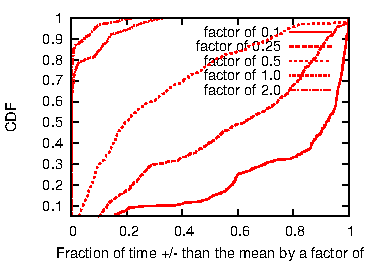
\includegraphics[width=0.4\textwidth] {figures/spatial-similarity.pdf}
\tightcaption{Spatial similarity of quality (average bitrate) among the sample of [Initial CDN, Initial Bitrate, ASN, Site, ConnectionType, Object].}
\label{fig:spatial-similarity}
\end{figure}

\myparasum{Spatial similarity} Spatial similarity is between the quality samples collected at the same time interval from sessions that share certain attribute values. \jc{Figure: x-Fraction of time less/greater than mean by various factor, y: CDF}

\begin{figure}[h!]
\centering
 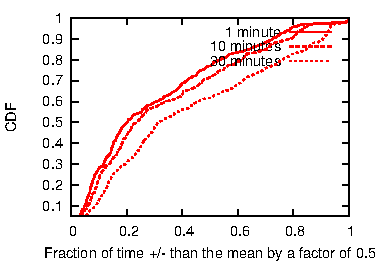
\includegraphics[width=0.4\textwidth] {figures/temporal-similarity.pdf}
\tightcaption{Quantifying impact of temporal noise on quality similarity. Figure shows likelihood of being more than a factor of 0.5 away from mean quality for all [Initial CDN, Initial Bitrate, ASN, Site, ConnectionType, Object] groups with increasing (from left to right) time scales.}
\label{fig:temporal-similarity}
\end{figure}

\myparasum{Temporal similarity} Temporal similarity is between the average quality collected in different time interval of the same group of sessions that share certain attribute values. \jc{Figure: x-Fraction of time less/greater than mean by various factor, y: CDF}

\myparasum{Summary of key observations} \jc{mostly based on my previous experience. subject to change after formal results are generated.}
\begin{packedenumerate}
	\item Both similarity of quality samples show that it is feasible to predict the quality of a new session and its decision by looking at quality samples that are spatially and temporally close to it.
	\item Spatial similarity varies across different attributes.  Using more attributes can improve things.
	\item Different quality metrics have different level of similarity, especially, buffering ratio has the largest similarity.
\end{packedenumerate}

\tightsubsection{Predicting from finite data}
Unfortunately, we do not have access to infinite data.  This is problematic because the mean quality outcome of a small sample of similar sessions (for example, $10$ such sessions) is subject to considerable random noise.  If we use that number for prediction, the prediction will be subject to the same noise and consequently to high average error.  As the number of attributes grows, quality grows more predictable (as we have seen) but the number of perfectly-matched sessions may drop exponentially.

Of course, prediction in the presence of limited information is the domain of statistics, and there are many potential solutions to this problem.  Any solution will deal with, and potentially trade off, four sources of prediction error:


\begin{figure}[h!]
\centering
\subfigure[Prediction error vs. group size (w.r.t average bitrate)]
{
        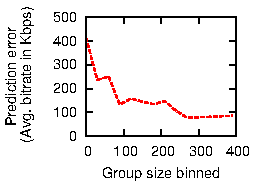
\includegraphics[width=110pt]{figures/count-err.pdf}
}
\subfigure[Distribution of group size]
{
        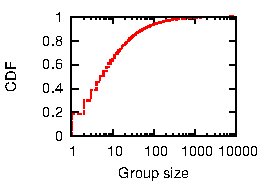
\includegraphics[width=110pt]{figures/count-cdf.pdf}
}
\tightcaption{Impact of group size (i.e., number of samples in a group). They show that more samples give more accuracy, and most of groups do not have sufficient samples for accurate prediction.}
\label{fig:group-size-impact}
\end{figure}

\begin{packedenumerate}
  \item \emph{Estimation error:} In the statistical literature, prediction error due to limited data is often called {\it estimation error}.  Other things being equal, more data produce more accurate prediction. For example, Figure~\ref{fig:group-size-impact}-(a) presents the prediction error of using a group as a function of its (i.e., number of samples). To show  In fact, estimation error is a serious practical problem for video quality prediction.  Using all available attributes, many sessions have very few matches, as we would expect given the exponential explosion in combinations of attribute values.  
  \item \emph{Bias} due to missing or unused information: When grouping sessions according to attributes we observe, we of course may not observe attributes that are important for prediction.  Say we do not observe (or use) important attribute X.  Then, even if we have infinitely many sessions that match the current session on all observed attributes, the average outcome for all of those sessions may be different from the average outcome for the subset of sessions that match the current session on attribute X.  This is a form of bias.  Predictability, as we have defined it, simply means low bias.  Importantly, it is not alleviated by gathering more session data; as we have seen, it may be alleviated by gathering more attributes about each session.
  \item \emph{Unavailability of recent data:} In a practical system, there are delays in sending and processing quality samples, so they are not available instantly.  If conditions change rapidly, there may be no quality samples sufficiently close to the session under prediction.  This is an extreme example of estimation error.  In this case it may be necessary to model the evolution of the video ecosystem over time in order to extrapolate to the current time.

\begin{figure}[h!]
\centering
 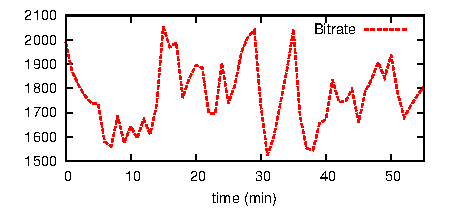
\includegraphics[width=0.4\textwidth] {figures/quality-time.pdf}
\tightcaption{Temporal variability of quality. The figure shows the mean value of average bitrate of a fixed group of same [Site, Initial CDN, Initial Bitrate, ConnectionType, ASN, Object], which has 100 quality samples in every minute in the figure.}
\label{fig:quality-variability}
\end{figure}

  \item \emph{Noise:} Even if we observed all conceivable attributes of a session and had infinitely many examples of exactly quality samples, outcomes may be affected by inputs that are practically random.  For example, performance may be affected by randomized algorithms in the networking layer.  This implies that some degree of prediction error is inevitable.
\end{packedenumerate}

More formally, we can derive this as follows (see \cite{domingos2000unified} for a less specialized discussion of the decomposition of prediction error).  Let $D$ be a set of quality samples from which a prediction algorithm learns its predictions.  Let $p_i$ be predicted quality for session $i$ and $q_i$ be its actual quality.  We further assume that $q_i$ is fixed except for an independent additive noise component, i.e. $q_i = \hat{q}_i + \epsilon_i$, where $\hat{q}_i$ is nonrandom and $\epsilon_i$ is a random variable with mean $0$, independent of $p_i$.  Then the expected squared prediction error, with respect to randomness in the observed data $D$ used to compute $p_i$, is:
\begin{align*}
  \E_D[(p_i - q_i)^2] &= \Var_D[p_i - q_i] + (\E_D[p_i - q_i])^2 \\
  &= \Var_D[p_i - \hat{q}_i - \epsilon_i] + (\E_D[p_i - \hat{q}_i - \epsilon_i])^2 \\
  &= \Var_D[p_i - \hat{q}_i] + \Var_D[\epsilon_i] + (\E_D[p_i - \hat{q}_i - \epsilon_i])^2\\
  &= \Var_D[p_i] + \Var_D[\epsilon_i] + (\E_D[p_i - \hat{q}_i - \epsilon_i])^2\\
  &= \Var_D[p_i] + \Var_D[\epsilon_i] + (\E_D[p_i - \hat{q}_i] - \E_D[\epsilon_i])^2\\
  &= \Var_D[p_i] + \Var_D[\epsilon_i] + (\E_D[p_i] - \hat{q})^2
\end{align*}

The first term is estimation error -- the variability in predictions across possible sets of observed data.  It will increase as the number of sessions similar to session $i$ in $D$ decreases; as a special case it may be very large if only a few quality samples in $D$ are temporally close to session $i$.  The second term is noise.  The third term is the squared bias of the predictor, which does not generally decrease with the size of $D$.  The prediction algorithm's average prediction error is simply the average over all sessions $i$ of the sum of these three terms.

\tightsubsection{Aggregation}
A simple strategy to reduce estimation error is {\it aggregation}.  By aggregation we mean putting sessions into coarser groups that match on only a subset of observed attributes.  Aggregation increases the number of samples in each group but reduces the number of attributes, thus reducing estimation error at the cost of increased bias.  Thus it makes sense to look for an optimal degree of aggregation.  Figures \fillme show that the optimal AC (the aggregation that gives minimal prediction error) is in many cases neither the finest nor the coarsest one.



\begin{figure}[h!]
\centering
 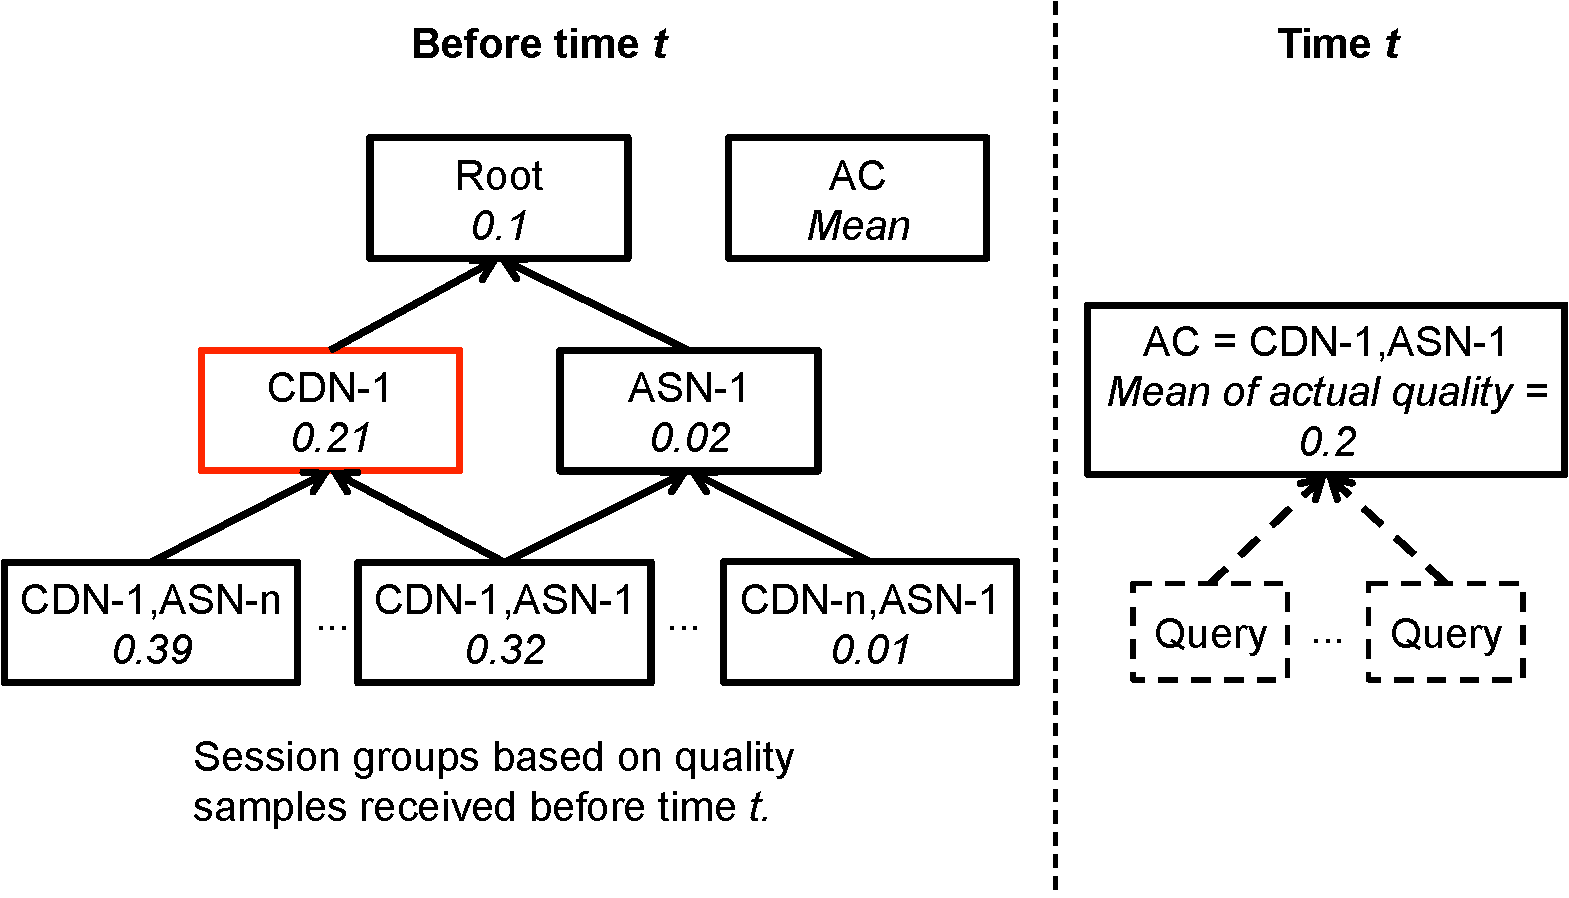
\includegraphics[width=0.5\textwidth] {figures/fig-optimal-AC.pdf}
\tightcaption{Example of how optimal AC is identified. The optimal AC is colored in red. Assuming the considered attributes are fixed, the optimal AC assumes that all sessions that belong to the same finest group should be given the same prediction, and the optimal AC is the one that gives the closest prediction among those that contain this finest group.}
\label{fig:example-optimal-ac}
\end{figure}

Figure~\fillme-(a) shows for each AC, the fraction of sessions for which it is the optimal AC with respect to average bitrate. We use ``CDN, starting bitrate, connection type, ASN'' as attributes and always look at one-minute history, in order to avoid impact of temporal aggregation. The figure shows that there is no dominant AC that is optimal for most of the sessions; Even the top five most frequent optimal ACs only count for less than \fillme of sessions. Figure~\fillme-(b) shows the frequency of the top five most frequent optimal AC over the period of \fillme hours. The figure shows that their frequency also changes with substential variability, which suggests that optimal AC must be chosen adaptively.
Therefore, there is no universal optimal AC or a set of ACs that can produce best prediction for even most of sessions. Moreover, in most cases, the optimal AC is neither the finest nor the coarsest AC.



\begin{figure}[h!]
\centering
\subfigure[Distribution of optimal AC. No single or small set of ACs can be used as optimal AC for most quries.]
{
        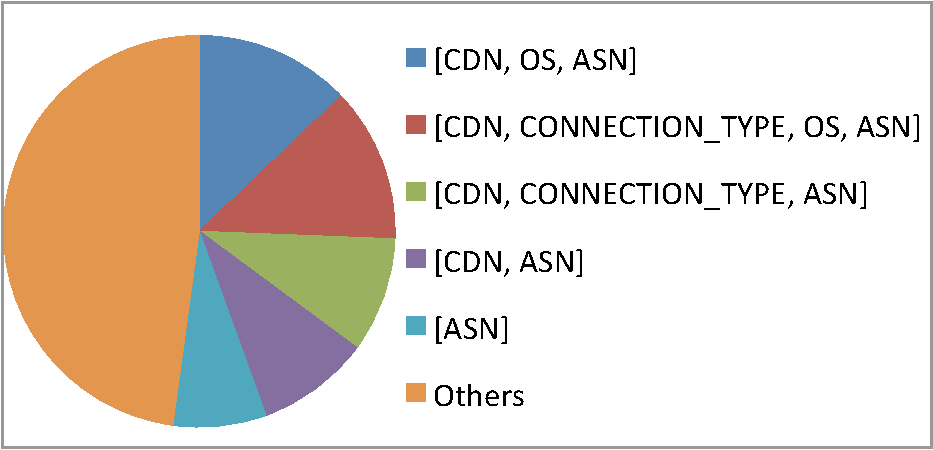
\includegraphics[width=0.4\textwidth]{figures/optimal_AC_distribution.pdf}
}
\subfigure[Prevalence of pair of (finest group, optimal AC). 70\% pairs of (finest group, optimal AC) only last for less than 20\% of time.]
{
        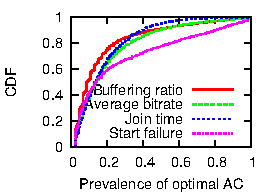
\includegraphics[width=0.4\textwidth]{figures/optimal-prevalence.pdf}
}
\tightcaption{Dynamics of the optimal AC. Prevalence of pair of (finest group, optimal AC) is the fraction of time that the finest group has this optimal AC.}
\label{fig:optimal-ac-dynamics}
\end{figure}

When estimation error is small (say, when a fine-grained group contains many sessions) we want to eliminate bias by using a fine-grained group.  When estimation error is large, we want to aggregate more.  Figure \fillme demonstrates this for \fillme.  This indicates that a prediction algorithm that uses aggregation should pay attention to its error rate to determine the right degree of aggregation.